\documentclass[a4paper, 10pt]{article}
\usepackage[top=0.5in, bottom=0.5in, left=1in, right=1in]{geometry}
% \usepackage[utf8]{inputenc}
% \usepackage[slantfont,boldfont]{xeCJK}
\usepackage{xeCJK}

\usepackage{fontspec}
% \setCJKmainfont{Noto Sans CJK SC}
% \setCJKmainfont{Noto Sans CJK SC Regular}
% \setCJKmainfont[BoldFont=SimHei, ItalicFont=KaiTi]{SimSun}
\setCJKmonofont[BoldFont=SimHei, ItalicFont=KaiTi]{SimSun}
% \setCJKmainfont{AR PL UMing CN}
\setmainfont{Times New Roman}
% \setmainfont{Arial}
% \setsansfont{Arial}
\usepackage{latexsym}
\usepackage{amsmath,amssymb,amsfonts}
\usepackage{color,xcolor}
\usepackage{graphicx}
\usepackage{caption}
\usepackage{subcaption}
\usepackage{tabu}
\usepackage{booktabs}
\usepackage{bm}
\usepackage{footnote}
\usepackage{url}
% \usepackage{subcaptionbox}
% \usepackage{subfigure}


\newcommand{\bX}{\mathbf{X}}
\newcommand{\bY}{\mathbf{Y}}
\newcommand{\bZ}{\mathbf{Z}}
\newcommand{\bH}{\mathbf{H}}





\title{2D人体骨架识别}
\author{
安亮\\
2017310876
\and
秦钰超(coauthor)\\
2017210955
}
\begin{document}
\maketitle
\pagestyle{plain}
\setlength{\parindent}{2em}
\makeatletter
\renewcommand{\section}{\@startsection{section}{1}{0mm}
{0.5\baselineskip}{0.5\baselineskip}
{\Large\bf\leftline}}
\makeatother

\renewcommand\thefigure{\thesection.\arabic{figure}}
\makeatletter
\@addtoreset{figure}{section}
\makeatother


\section{摘要}
本工作参考VNect实现了一个用于2D人体骨架检测的巻积神经网络。在测试数据上,该网络能够对部分人体关节点实现比较准确的检测。代码参见github\footnote{\url{https://github.com/anl13/Pose3D}}。

\section{研究问题}
人体骨架,又称人体关键点,指的是能反应人体姿态的关节点,例如肘、肩等。人体关键点检测(或人体骨架识别)指的是在一张或者多张图片
中,利用计算机算法标注出人体关键点在图像中的位置。这是计算机视觉领域广受关注的任务,也是实现人机交互的核心问题。
随着神经网络技术的广泛应用,利用神经网络解决诸如人体关键点检测等问题成为研究热点。CPM \cite{wei2016convolutional}首先实现了利用
巻积神经网络检测单人人体关键点,随后openpose\cite{cao2016realtime}成功使用巻积神经网络实现了单张图片多人体关节点检测。
最近,利用单张图片实现3D人体关键点检测也获得了很大关注,\cite{newell2016stacked}设计了特殊的巻积网络结构——stacked hourglass实现了较为
精确的单人体3D骨架识别。VNECT\cite{mehta2017vnect}则将2D人体关键点检测与坐标估计结合起来,实现了实时单人3D关键点检测与跟踪。

本工作研究的问题是单图片单人2D人体骨架检测问题。本工作参考VNECT中的2D骨架识别网络的网络结构,利用tensorflow\cite{abadi2016tensorflow}
予以实现,并在少量数据上进行了效果测试。

\section{采用数据}
本文主要采用的数据是mpi-inf-3dhp\cite{mehta2017monocular}。这是一个单人体数据集,带有2D和3D的关节标注。由于时间问题,本文并没有
利用该数据进行训练,而是直接迁移了VNECT训练出的模型参数,并在该数据集的个别图像上进行了测试。


\section{研究方法}

\subsection{网络结构}

\hspace{2em}本文使用了图\ref{pic:net_struct}展示了我们使用的网络结构。其中,我们最终利用的输出仅为H层,也就是2D关节点heatmap层。在这个网络中,针对每个关节点会输出一个heatmap,
heatmap上能量最高的位置就是该关节点出现概率最大的位置。因此,最终输出的heatmap张量的维度为(N,H,W,C),N是输入图像的数量(在测试的时候一般为1),H是和heatmap图像的高度
(在该网络中是输入图像的$1/8$,W相同),W是heatmap图像的高度,C是heatmap图像的通道数,在该网络中为21,对应待检测的关节点数量。

这个网络有两个优点。第一,网络的前端使用了ResNet\cite{he2016deep}作为特征提取器,通过迁移ResNet在imagenet上训练好的参数可以加速网络训练的收敛速度。
第二,使用了全巻积的结构(除了计算关节长度部分),使得网络适应任何大小的图片输入。

\begin{figure}[ht!]
    \centering
    \includegraphics[width=\linewidth]{pic/net_struct.png}
    \caption{网络结构。}
    \label{pic:net_struct}
\end{figure}

对于该网络,我们考虑直接把参数从VNECT网络训练出的参数迁移过来。然而,这里面也面临一些问题。原来的VNECT网络是用caffe架构训练出来的,参数表达的结构
也是caffe的结构。两种网络的参数在卷积核的维度顺序等方面有不少区别,我们在转换的时候进行了很多次尝试。然而,最终我们转移过来的参数并没有表现出完美的
结果,但仍然在部分关节的检测中展示出了不错的结果\footnote{这部分工作主要由秦钰超同学完成}。


\subsection{网络原理}

\hspace{2em}VNECT本身是基于ResNet50,通过使用后续的网络处理ResNet提取的图像特征实现对人体关节的2D和3D姿态识别,具体的网络设计如图\ref{pic:net_struct}所示。
方便起见,我们分别将通道$j$对应的$H$,$X$,$Y$,$Z$层的输出记为$\bH_j$,$\bX_j$,$\bY_j$,$\bZ_j$。

训练VNECT时,首先针对$H$层进行训练,使其能够正确给出人体的2D关节的heatmap。训练时对应的损失函数如式(\ref{eqn:h})所示,其中上标$GT$表示Ground Truth。
通过最小化式\ref{eqn:h}中定义的损失函数,网络输出的$H$层最终将给出正确的2D关节heatmap。
对3D关节的heatmap的训练在完成2D关节heatmap的训练后进行,此时的$H$层输出可以被当作Ground Truth使用。我们使用式(\ref{eqn:x})中定义的
损失函数对$X$层的输出进行训练,其中上标$GT$表示Ground Truth,$\odot$表示Hadamard product。$\bY_j$,$\bZ_j$层的训练也使用类似的损失函数进行。

\begin{eqnarray}
        Loss(h_j)&=& || \bH^{GT}_{j}-\bH_j ||_2 \label{eqn:h}\\
        Loss(x_j)&=& || \bH^{GT}_{j}\odot(\bX_j-\bX^{GT}_{j}) ||_2 \label{eqn:x}\\
        Loss(y_j)&=& || \bH^{GT}_{j}\odot(\bY_j-\bY^{GT}_{j}) ||_2 \label{eqn:y}\\
        Loss(z_j)&=& || \bH^{GT}_{j}\odot(\bZ_j-\bZ^{GT}_{j}) ||_2 \label{eqn:z}
\end{eqnarray}


\subsection{数据处理}

\hspace{2em}为了使图片转换为神经网络容易处理的形势,我们对图像进行了预处理和后处理\footnote{这部分工作主要由我完成}。

在预处理方面,考虑到我们的神经网络输出的heatmap的宽和高是输入图像的$1/8$,为了对输出图像做更好的处理,对于一个输入的图像$I$,我们首先会对图像进行尺度上的放缩,
将宽和高放缩到8的整数倍。其次,原输入图像每个像素点的值的范围是$(0,255)$,这种过大的取值范围对于神经网络是不友好的。因此,我们将像素点的值放缩到$(-0.4,0.6)$。

在后处理方面,我们将heatmap的尺度和值范围还原到原图,并提取heatmap最大值的坐标作为关节估计位置。

\section{结果分析}
我们将图\ref{pic:input}中的图片输入到我们重新构建的VNCET网络中,网络的输出经过后处理得到的2D人体关节识别结果如图\ref{pic:result}所示。
可以看到我们使用tensorflow搭建的网络成功地识别出了相当数量的关节,同时也有一部分关节的位置则出现了明显的错误。
而实际运行原始的caffe模型得到的结果则非常优秀,每一个人体关节都被正确地标识了出来。我们重新构建的网络和原始的caffe网络使用的参数完全一致,
我们猜想可能是tensorflow和caffe框架对于VNECT使用到的卷积层等结构的实现上的差异导致了这一结果上的不同。
在tensorflow框架下对参数进行微调可能会得到更好的结果。

\begin{figure}[!ht]
        \begin{subfigure}[b]{0.48\linewidth}
                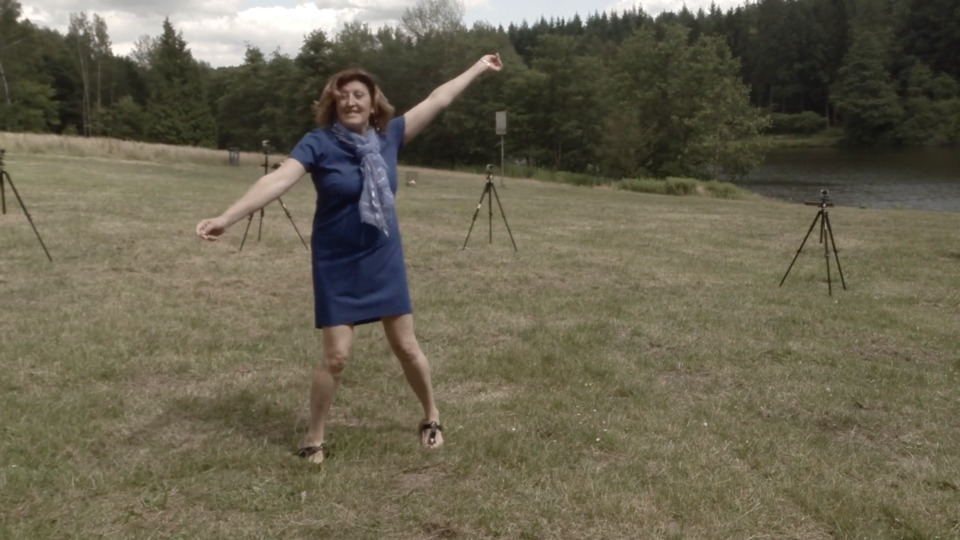
\includegraphics[width=\linewidth]{pic/input.jpg}
                \caption{输入图片}
                \label{pic:input}
        \end{subfigure}
        \hfill
        \begin{subfigure}[b]{0.48\linewidth}
                \includegraphics[width=\linewidth]{pic/result.png}
                \caption{2D关节识别结果}
                \label{pic:result}
        \end{subfigure}
        \caption{VNECT网络识别结果}
\end{figure}

\begin{figure}[!ht]
        \begin{subfigure}[b]{0.48\linewidth}
                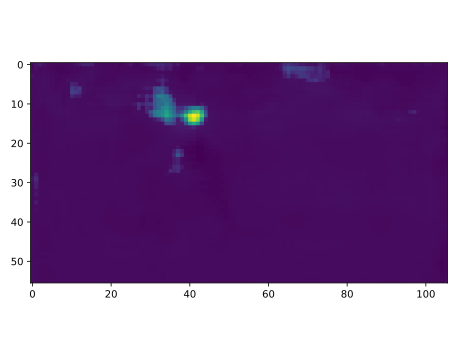
\includegraphics[width=\linewidth]{pic/good_heatmap_5.pdf}
                \caption{通道5的heatmap}
                \label{pic:good5}
        \end{subfigure}
        \hfill
        \begin{subfigure}[b]{0.48\linewidth}
                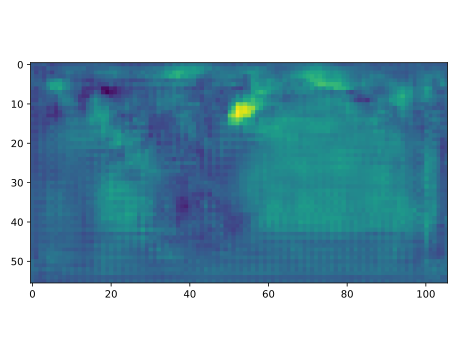
\includegraphics[width=\linewidth]{pic/good_heatmap_12.pdf}
                \caption{通道12的heatmap}
                \label{pic:good12}
        \end{subfigure}
        \caption{VNECT网络较好的输出结果\label{pic:good}}
\end{figure}

\begin{figure}[!ht]
        \begin{subfigure}[b]{0.48\linewidth}
                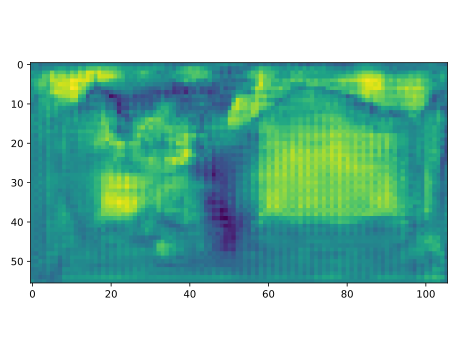
\includegraphics[width=\linewidth]{pic/bad_heatmap_15.pdf}
                \caption{通道15的heatmap}
                \label{pic:bad15}
        \end{subfigure}
        \hfill
        \begin{subfigure}[b]{0.48\linewidth}
                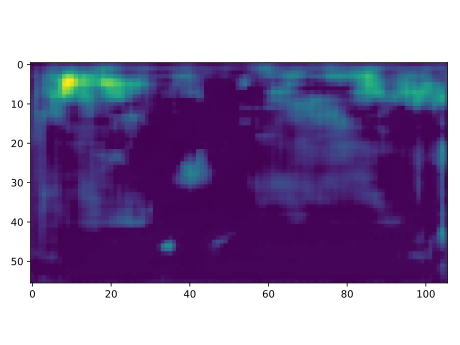
\includegraphics[width=\linewidth]{pic/bad_heatmap_19.pdf}
                \caption{通道19的heatmap}
                \label{pic:bad19}
        \end{subfigure}
        \caption{VNECT网络较差的输出结果 \label{pic:bad}}
\end{figure}

我们选择VNECT网络输出的$H$层的部分典型通道进行对比分析。图\ref{pic:good}显示了其中的通道5(\ref{pic:good5})
和通道12(\ref{pic:good5})的heatmap。容易看出,这两个通道给出的heatmap清晰地给出了对应的关节(肩、手腕)在图中对应的位置。
虽然有很多通道给出的heatmap和\ref{pic:good}非常类似,能够给出非常好的识别结果,但是也有一些通道的heatmap存在很强的干扰,
如图\ref{pic:bad}所示。可以看到,通道15和通道19的heatmap虽然都在脚踝处出现了局部的极大值,其他位置出现的干扰却使得后处理算法给出了错误的关节位置,这
种噪声在\ref{pic:bad15}中显得尤其严重。如同前面提到的,这一问题应该是caffe和tensorflow在实现上的差异导致的,通过在训练数据集上进行参数微调应该可以解决。

\section{主要贡献}
本人在此课程Project中的主要贡献如下:
\begin{itemize}
        \item 图像处理。
        \item 部分网络调试与分析。
        \item 图像理解。
\end{itemize}




\bibliographystyle{splncs}
\bibliography{ref.bib}

\end{document}
